% ============================================================
% CHAPTER 6: VISION TRANSFORMER (ViT)
% Deep Expert Analysis - Main Focus Chapter
% ============================================================
\chapter{Vision Transformer (ViT)}

\section{Motivation: From NLP to Vision}

\subsection{The Transformer Revolution}

\begin{tcolorbox}[colback=blue!5!white,colframe=blue!75!black,title=Historical Context]
\textbf{2017:} ``Attention Is All You Need'' (Vaswani et al.)
\begin{itemize}
    \item Transformer thay thế RNN trong NLP
    \item Self-attention captures long-range dependencies
    \item Parallelizable → faster training
\end{itemize}

\textbf{2020:} ``An Image is Worth 16×16 Words'' (Dosovitskiy et al.)
\begin{itemize}
    \item Áp dụng Transformer pure cho vision
    \item Images = sequences of patches
    \item State-of-the-art khi pretrained on large data
\end{itemize}
\end{tcolorbox}

\subsection{Paper Motivation}

\paperref{Section 3.3 - Vision Transformer}

\begin{tcolorbox}[colback=yellow!5!white,colframe=yellow!75!black,title=Paper Quote - ViT Motivation]
\textit{``Vision Transformer (ViT) [3] follows an approach to image classification by treating an image as a sequence of patches and processing it using a standard Transformer encoder like the ones used in NLP.''}
\end{tcolorbox}

\subsection{CNN vs Transformer Inductive Biases}

\begin{table}[H]
\centering
\caption{Inductive Biases: CNN vs ViT}
\begin{tabular}{lcc}
\toprule
\textbf{Inductive Bias} & \textbf{CNN} & \textbf{ViT} \\
\midrule
Locality & \checkmark Strong & \texttimes Weak \\
Translation Equivariance & \checkmark Built-in & \texttimes Learned \\
2D Structure & \checkmark Preserved & \texttimes Flattened \\
Long-range Dependencies & \texttimes Limited & \checkmark Global \\
Data Efficiency & \checkmark Good & \texttimes Needs more data \\
Scalability & Limited & \checkmark Scales well \\
\bottomrule
\end{tabular}
\end{table}

\section{ViT Architecture Overview}

\begin{figure}[H]
\centering
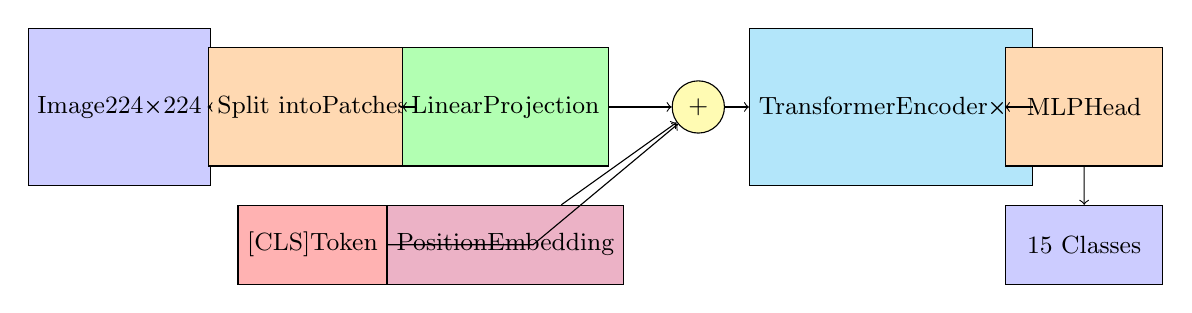
\begin{tikzpicture}[scale=0.7, every node/.style={font=\small}]
    % Input image
    \node[draw, fill=blue!20, minimum width=2cm, minimum height=2cm] (img) at (0,0) {Image\\224×224};
    
    % Patches
    \node[draw, fill=orange!30, minimum width=2cm, minimum height=1.5cm] (patch) at (3.5,0) {Split into\\Patches};
    
    % Linear projection
    \node[draw, fill=green!30, minimum width=2cm, minimum height=1.5cm] (proj) at (7,0) {Linear\\Projection};
    
    % Position embedding
    \node[draw, fill=purple!30, minimum width=2cm, minimum height=1cm] (pos) at (7,-2.5) {Position\\Embedding};
    
    % CLS token
    \node[draw, fill=red!30, minimum width=1.5cm, minimum height=1cm] (cls) at (3.5,-2.5) {[CLS]\\Token};
    
    % Add
    \node[draw, circle, fill=yellow!30] (add) at (10.5,0) {+};
    
    % Transformer Encoder
    \node[draw, fill=cyan!30, minimum width=2.5cm, minimum height=2cm] (trans) at (14,0) {Transformer\\Encoder\\×L};
    
    % MLP Head
    \node[draw, fill=orange!30, minimum width=2cm, minimum height=1.5cm] (mlp) at (17.5,0) {MLP\\Head};
    
    % Output
    \node[draw, fill=blue!20, minimum width=2cm, minimum height=1cm] (out) at (17.5,-2.5) {15 Classes};
    
    % Arrows
    \draw[->] (img) -- (patch);
    \draw[->] (patch) -- (proj);
    \draw[->] (proj) -- (add);
    \draw[->] (pos) -- (add);
    \draw[->] (cls) -- ++(4,0) -- (add);
    \draw[->] (add) -- (trans);
    \draw[->] (trans) -- (mlp);
    \draw[->] (mlp) -- (out);
\end{tikzpicture}
\caption{Vision Transformer Architecture Overview}
\end{figure}

\section{Step 1: Patch Embedding}

\subsection{Concept}

\paperref{Section 3.3 - Vision Transformer}

\begin{tcolorbox}[colback=yellow!5!white,colframe=yellow!75!black,title=Paper Quote - Patch Embedding]
\textit{``This involves dividing the image into fixed-size non-overlapping patches, which are then linearly embedded. In our experiments, we fix a patch size of 32 × 32 for all our Vision Transformer models.''}
\end{tcolorbox}

\subsection{Toán học}

Với image $x \in \mathbb{R}^{H \times W \times C}$ và patch size $P$:

\textbf{Step 1: Chia patch}
\begin{equation}
\text{Number of patches: } N = \frac{H \times W}{P^2} = \frac{224 \times 224}{32 \times 32} = 49
\end{equation}

\textbf{Step 2: Flatten mỗi patch}
\begin{equation}
x_p^i \in \mathbb{R}^{P^2 \cdot C} = \mathbb{R}^{32 \times 32 \times 3} = \mathbb{R}^{3072}
\end{equation}

\textbf{Step 3: Linear projection}
\begin{equation}
z_0^i = x_p^i \cdot E + b, \quad E \in \mathbb{R}^{(P^2 \cdot C) \times D}
\end{equation}

Trong đó $D$ là embedding dimension (projection\_dim = 64 trong paper).

\subsection{Implementation trong Code}

\coderef{ViT-v1.ipynb}

\begin{lstlisting}[caption={PatchEmbedding Class - Phiên bản 1}]
class PatchEmbedding(nn.Module):
    """
    Convert image into patch embeddings.
    
    Paper: "dividing the image into fixed-size non-overlapping patches"
    Implementation: Use Conv2d with kernel_size=stride=patch_size
    """
    def __init__(self, img_size=224, patch_size=32, in_channels=3, embed_dim=64):
        super(PatchEmbedding, self).__init__()
        self.img_size = img_size
        self.patch_size = patch_size
        self.num_patches = (img_size // patch_size) ** 2  # 49 patches
        
        # ===== Linear Projection via Conv2d =====
        # Equivalent to: flatten patch -> linear layer
        # But more efficient implementation
        self.projection = nn.Conv2d(
            in_channels=in_channels,   # 3 (RGB)
            out_channels=embed_dim,    # 64 (projection_dim)
            kernel_size=patch_size,    # 32x32
            stride=patch_size          # Non-overlapping
        )
        
    def forward(self, x):
        # x: (B, 3, 224, 224)
        
        # Apply projection
        x = self.projection(x)
        # Shape: (B, embed_dim, num_patches_h, num_patches_w)
        # = (B, 64, 7, 7)
        
        # Flatten spatial dimensions
        x = x.flatten(2)
        # Shape: (B, 64, 49)
        
        # Transpose to (B, num_patches, embed_dim)
        x = x.transpose(1, 2)
        # Shape: (B, 49, 64)
        
        return x
\end{lstlisting}

\subsection{Tại sao dùng Conv2d cho Linear Projection?}

\begin{tcolorbox}[colback=green!5!white,colframe=green!75!black,title=Conv2d = Efficient Linear Projection]
\textbf{Method 1: Naive (unfold + linear)}
\begin{lstlisting}[style=plain]
patches = x.unfold(2, P, P).unfold(3, P, P)  # Extract patches
patches = patches.reshape(B, N, P*P*C)       # Flatten
embeddings = linear(patches)                  # Project
\end{lstlisting}

\textbf{Method 2: Conv2d (elegant)}
\begin{lstlisting}[style=plain]
embeddings = conv2d(x, kernel=P, stride=P)   # One operation!
\end{lstlisting}

\textbf{Equivalence:} Conv2d với kernel\_size=stride=P chính là:
\begin{itemize}
    \item Extract non-overlapping patches
    \item Apply same linear transformation to each patch
    \item Output: one value per patch per filter = embedding
\end{itemize}
\end{tcolorbox}

\section{Step 2: Positional Embedding}

\subsection{Tại sao cần Position Information?}

\begin{tcolorbox}[colback=red!5!white,colframe=red!75!black,title=Problem: Self-Attention is Permutation Invariant]
Self-attention treats input as a \textbf{set}, not a \textbf{sequence}.

\textbf{Ví dụ:} Với patches $[p_1, p_2, p_3]$:
\begin{itemize}
    \item Attention($[p_1, p_2, p_3]$) = Attention($[p_3, p_1, p_2]$)
    \item Model không biết patch nào ở đâu!
    \item Vị trí quan trọng: lung ở giữa, heart ở trái
\end{itemize}

\textbf{Solution:} Add positional information to embeddings.
\end{tcolorbox}

\subsection{Learnable vs Fixed Positional Embedding}

\begin{table}[H]
\centering
\caption{Positional Embedding Types}
\begin{tabular}{lp{5cm}p{5cm}}
\toprule
\textbf{Type} & \textbf{Sinusoidal (Fixed)} & \textbf{Learnable} \\
\midrule
Formula & $PE_{pos,2i} = \sin(pos/10000^{2i/d})$ & Random init, trained \\
Parameters & 0 & $N \times D$ \\
Generalization & To any length & Fixed length \\
ViT choice & - & \checkmark Used \\
\bottomrule
\end{tabular}
\end{table}

\subsection{Implementation}

\begin{lstlisting}[caption={Positional Embedding trong ViT}]
class VisionTransformer(nn.Module):
    def __init__(self, ...):
        # ...
        
        # ===== Positional Embedding =====
        # Paper: "learnable 1D position embeddings"
        # Shape: (1, num_patches + 1, embed_dim) = (1, 50, 64)
        # +1 for CLS token
        self.pos_embedding = nn.Parameter(
            torch.randn(1, num_patches + 1, embed_dim)
        )
        
    def forward(self, x):
        # After patch embedding: (B, 49, 64)
        
        # Add CLS token
        cls_tokens = self.cls_token.expand(B, -1, -1)  # (B, 1, 64)
        x = torch.cat([cls_tokens, x], dim=1)          # (B, 50, 64)
        
        # Add positional embedding
        x = x + self.pos_embedding  # (B, 50, 64) + (1, 50, 64) broadcast
        
        return x
\end{lstlisting}

\section{Step 3: [CLS] Token}

\subsection{Origin: BERT}

\begin{tcolorbox}[colback=blue!5!white,colframe=blue!75!black,title=CLS Token Concept]
\textbf{Nguồn gốc:} BERT (NLP)
\begin{itemize}
    \item Special token prepended to input sequence
    \item Learns to aggregate information from all tokens
    \item Used for classification tasks
\end{itemize}

\textbf{Trong ViT:}
\begin{itemize}
    \item Prepend một learnable token trước patch embeddings
    \item Sau Transformer: CLS token ``nhìn'' toàn bộ image
    \item Dùng CLS token cho final classification
\end{itemize}
\end{tcolorbox}

\subsection{Implementation}

\begin{lstlisting}[caption={CLS Token Implementation}]
class VisionTransformer(nn.Module):
    def __init__(self, ...):
        # ===== CLS Token =====
        # Learnable parameter
        # Shape: (1, 1, embed_dim) = (1, 1, 64)
        self.cls_token = nn.Parameter(
            torch.zeros(1, 1, embed_dim)
        )
        
    def forward(self, x):
        B = x.shape[0]
        
        # Patch embedding: (B, 49, 64)
        x = self.patch_embed(x)
        
        # Expand CLS token for batch
        cls_tokens = self.cls_token.expand(B, -1, -1)  # (B, 1, 64)
        
        # Concatenate: CLS + patches
        x = torch.cat([cls_tokens, x], dim=1)  # (B, 50, 64)
        # Position 0 = CLS, Positions 1-49 = patches
        
        # After Transformer encoder...
        x = self.transformer(x)  # (B, 50, 64)
        
        # Extract CLS token for classification
        cls_output = x[:, 0]  # (B, 64) - first token
        
        return self.head(cls_output)
\end{lstlisting}

\section{Step 4: Transformer Encoder}

\subsection{Self-Attention Mechanism}

\paperref{Section 3.3 - Vision Transformer}

\begin{tcolorbox}[colback=yellow!5!white,colframe=yellow!75!black,title=Paper Quote - Multi-Head Attention]
\textit{``Our Vision Transformer implementation includes Multi-Head Self-Attention (MHSA). It also includes MLP blocks and Layer Normalization (LN) applied before every block, and residual connections applied after every block.''}
\end{tcolorbox}

\subsubsection{Single-Head Attention}

\begin{equation}
\text{Attention}(Q, K, V) = \text{softmax}\left(\frac{QK^T}{\sqrt{d_k}}\right) V
\end{equation}

Trong đó:
\begin{itemize}
    \item $Q = XW^Q$ (Queries): ``What am I looking for?''
    \item $K = XW^K$ (Keys): ``What do I contain?''
    \item $V = XW^V$ (Values): ``What information do I provide?''
    \item $\sqrt{d_k}$: Scaling factor để ổn định gradient
\end{itemize}

\begin{figure}[H]
\centering
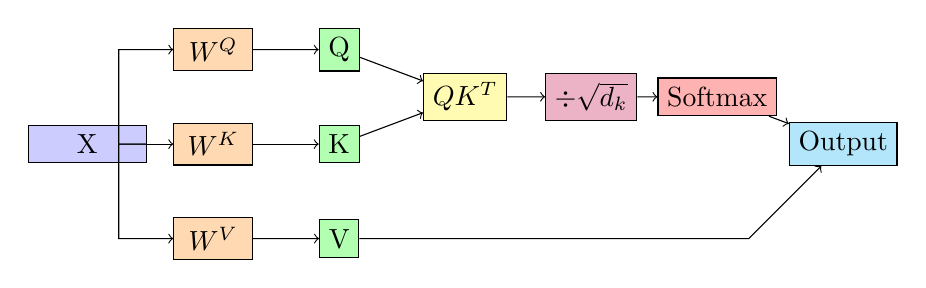
\begin{tikzpicture}[scale=0.8]
    % Input
    \node[draw, fill=blue!20, minimum width=1.5cm] (x) at (0,0) {X};
    
    % Q, K, V projections
    \node[draw, fill=orange!30, minimum width=1cm] (wq) at (2,1.5) {$W^Q$};
    \node[draw, fill=orange!30, minimum width=1cm] (wk) at (2,0) {$W^K$};
    \node[draw, fill=orange!30, minimum width=1cm] (wv) at (2,-1.5) {$W^V$};
    
    % Q, K, V
    \node[draw, fill=green!30] (q) at (4,1.5) {Q};
    \node[draw, fill=green!30] (k) at (4,0) {K};
    \node[draw, fill=green!30] (v) at (4,-1.5) {V};
    
    % MatMul QK
    \node[draw, fill=yellow!30] (qk) at (6,0.75) {$QK^T$};
    
    % Scale
    \node[draw, fill=purple!30] (scale) at (8,0.75) {$\div\sqrt{d_k}$};
    
    % Softmax
    \node[draw, fill=red!30] (soft) at (10,0.75) {Softmax};
    
    % MatMul with V
    \node[draw, fill=cyan!30] (out) at (12,0) {Output};
    
    % Arrows
    \draw[->] (x) -- ++(0.5,0) -- ++(0,1.5) -- (wq);
    \draw[->] (x) -- (wk);
    \draw[->] (x) -- ++(0.5,0) -- ++(0,-1.5) -- (wv);
    
    \draw[->] (wq) -- (q);
    \draw[->] (wk) -- (k);
    \draw[->] (wv) -- (v);
    
    \draw[->] (q) -- (qk);
    \draw[->] (k) -- (qk);
    \draw[->] (qk) -- (scale);
    \draw[->] (scale) -- (soft);
    \draw[->] (soft) -- (out);
    \draw[->] (v) -- ++(6.5,0) -- (out);
\end{tikzpicture}
\caption{Scaled Dot-Product Attention}
\end{figure}

\subsubsection{Multi-Head Attention}

\begin{equation}
\text{MultiHead}(Q, K, V) = \text{Concat}(\text{head}_1, ..., \text{head}_h) W^O
\end{equation}

\begin{equation}
\text{head}_i = \text{Attention}(QW_i^Q, KW_i^K, VW_i^V)
\end{equation}

\begin{tcolorbox}[colback=green!5!white,colframe=green!75!black,title=Why Multi-Head?]
\begin{itemize}
    \item Mỗi head có thể attend to different aspects
    \item Head 1: positional relationships
    \item Head 2: color similarities
    \item Head 3: shape patterns
    \item Concatenate → richer representation
\end{itemize}
\end{tcolorbox}

\subsection{Implementation}

\coderef{ViT-v1.ipynb}

\begin{lstlisting}[caption={TransformerEncoderBlock Implementation}]
class TransformerEncoderBlock(nn.Module):
    """
    Single Transformer Encoder block.
    
    Architecture:
        x -> LayerNorm -> MHSA -> + -> LayerNorm -> MLP -> + -> output
             |__________________|      |_______________|
                 Skip connection          Skip connection
    """
    def __init__(self, embed_dim, num_heads, mlp_ratio=4.0, dropout=0.1):
        super(TransformerEncoderBlock, self).__init__()
        
        # ===== Layer Normalization (Pre-Norm) =====
        # Paper: "Layer Normalization applied before every block"
        self.norm1 = nn.LayerNorm(embed_dim)
        self.norm2 = nn.LayerNorm(embed_dim)
        
        # ===== Multi-Head Self-Attention =====
        # Paper: "Multi-Head Self-Attention (MHSA)"
        self.attn = nn.MultiheadAttention(
            embed_dim=embed_dim,   # 64
            num_heads=num_heads,   # 4 heads -> head_dim = 16
            dropout=dropout,
            batch_first=True       # Input: (B, N, D)
        )
        
        # ===== MLP Block =====
        # Paper: "MLP blocks"
        mlp_hidden_dim = int(embed_dim * mlp_ratio)  # 64 * 4 = 256
        self.mlp = MLP(
            in_features=embed_dim,
            hidden_features=mlp_hidden_dim,
            out_features=embed_dim,
            dropout=dropout
        )
        
        self.dropout = nn.Dropout(dropout)
        
    def forward(self, x):
        # ===== Attention Block with Skip Connection =====
        # Pre-LayerNorm (ViT uses pre-norm, not post-norm)
        attn_input = self.norm1(x)
        
        # Multi-Head Self-Attention
        # Query = Key = Value = same input (self-attention)
        attn_output, _ = self.attn(
            query=attn_input,
            key=attn_input,
            value=attn_input
        )
        
        # Skip connection (residual)
        x = x + self.dropout(attn_output)
        
        # ===== MLP Block with Skip Connection =====
        mlp_input = self.norm2(x)
        mlp_output = self.mlp(mlp_input)
        
        # Skip connection
        x = x + self.dropout(mlp_output)
        
        return x
\end{lstlisting}

\subsection{MLP Block}

\begin{lstlisting}[caption={MLP Block (Feed-Forward Network)}]
class MLP(nn.Module):
    """
    MLP block in Transformer.
    
    Architecture: Linear -> GELU -> Dropout -> Linear -> Dropout
    """
    def __init__(self, in_features, hidden_features, out_features, dropout=0.1):
        super(MLP, self).__init__()
        
        self.fc1 = nn.Linear(in_features, hidden_features)  # 64 -> 256
        self.act = nn.GELU()  # Gaussian Error Linear Unit
        self.fc2 = nn.Linear(hidden_features, out_features)  # 256 -> 64
        self.dropout = nn.Dropout(dropout)
        
    def forward(self, x):
        x = self.fc1(x)
        x = self.act(x)
        x = self.dropout(x)
        x = self.fc2(x)
        x = self.dropout(x)
        return x
\end{lstlisting}

\subsubsection{GELU Activation}

\begin{equation}
\text{GELU}(x) = x \cdot \Phi(x) = x \cdot \frac{1}{2}\left[1 + \text{erf}\left(\frac{x}{\sqrt{2}}\right)\right]
\end{equation}

\begin{tcolorbox}[colback=blue!5!white,colframe=blue!75!black,title=GELU vs ReLU]
\begin{itemize}
    \item GELU: Smooth approximation of ReLU
    \item Có curvature tại 0 (không có kink như ReLU)
    \item Cho phép small negative values
    \item Standard trong Transformers (BERT, GPT, ViT)
\end{itemize}
\end{tcolorbox}

\section{Complete ViT Implementation}

\begin{lstlisting}[caption={Complete VisionTransformer Class}]
class VisionTransformer(nn.Module):
    """
    Vision Transformer for Chest X-ray Classification.
    
    Paper configuration:
        - patch_size: 32 (ViT-v1/32)
        - embed_dim: 64
        - depth: 8 transformer blocks
        - num_heads: 4
        - mlp_ratio: 4.0
        - num_classes: 15
    """
    def __init__(
        self,
        img_size=224,
        patch_size=32,
        in_channels=3,
        num_classes=15,
        embed_dim=64,
        depth=8,
        num_heads=4,
        mlp_ratio=4.0,
        dropout=0.1
    ):
        super(VisionTransformer, self).__init__()
        
        # ===== Patch Embedding =====
        self.patch_embed = PatchEmbedding(
            img_size=img_size,
            patch_size=patch_size,
            in_channels=in_channels,
            embed_dim=embed_dim
        )
        num_patches = self.patch_embed.num_patches  # 49
        
        # ===== CLS Token =====
        self.cls_token = nn.Parameter(torch.zeros(1, 1, embed_dim))
        
        # ===== Positional Embedding =====
        # +1 for CLS token
        self.pos_embedding = nn.Parameter(
            torch.randn(1, num_patches + 1, embed_dim) * 0.02
        )
        
        self.pos_dropout = nn.Dropout(dropout)
        
        # ===== Transformer Encoder =====
        self.transformer = nn.Sequential(*[
            TransformerEncoderBlock(
                embed_dim=embed_dim,
                num_heads=num_heads,
                mlp_ratio=mlp_ratio,
                dropout=dropout
            )
            for _ in range(depth)  # 8 blocks
        ])
        
        # ===== Final LayerNorm =====
        self.norm = nn.LayerNorm(embed_dim)
        
        # ===== Classification Head =====
        self.head = nn.Linear(embed_dim, num_classes)
        
        # ===== Weight Initialization =====
        self._init_weights()
        
    def _init_weights(self):
        # Initialize cls_token
        nn.init.normal_(self.cls_token, std=0.02)
        
        # Initialize linear layers
        for m in self.modules():
            if isinstance(m, nn.Linear):
                nn.init.xavier_uniform_(m.weight)
                if m.bias is not None:
                    nn.init.zeros_(m.bias)
        
    def forward(self, x):
        B = x.shape[0]
        
        # 1. Patch Embedding: (B, 3, 224, 224) -> (B, 49, 64)
        x = self.patch_embed(x)
        
        # 2. Prepend CLS Token: (B, 49, 64) -> (B, 50, 64)
        cls_tokens = self.cls_token.expand(B, -1, -1)
        x = torch.cat([cls_tokens, x], dim=1)
        
        # 3. Add Positional Embedding
        x = x + self.pos_embedding
        x = self.pos_dropout(x)
        
        # 4. Transformer Encoder: (B, 50, 64) -> (B, 50, 64)
        x = self.transformer(x)
        
        # 5. Final Norm
        x = self.norm(x)
        
        # 6. Extract CLS Token: (B, 50, 64) -> (B, 64)
        cls_output = x[:, 0]
        
        # 7. Classification Head: (B, 64) -> (B, 15)
        output = self.head(cls_output)
        
        return output
\end{lstlisting}

\section{Paper Configurations: ViT-v1 vs ViT-v2}

\paperref{Section 4.2 - Models}

\begin{tcolorbox}[colback=yellow!5!white,colframe=yellow!75!black,title=Paper Quote - ViT Configurations]
\textit{``Vision Transformer v1 (32 × 32) (ViT-v1/32): our implementation of Vision Transformer with patch size 32 × 32 trained using our custom configuration (Table I).''}

\textit{``Vision Transformer v2 (32 × 32) (ViT-v2/32): our implementation of Vision Transformer with patch size 32 × 32 trained using (Section III-C) hyperparameter (Table III).''}
\end{tcolorbox}

\begin{table}[H]
\centering
\caption{ViT-v1 vs ViT-v2 Configurations}
\begin{tabular}{lcc}
\toprule
\textbf{Hyperparameter} & \textbf{ViT-v1} & \textbf{ViT-v2} \\
\midrule
Patch Size & 32 × 32 & 32 × 32 \\
Projection Dim & 64 & 64 \\
Transformer Layers & 8 & 8 \\
Attention Heads & 4 & 4 \\
MLP Head Units & [2048, 1024] & [2048, 1024] \\
Learning Rate & 0.001 & 0.0001 \\
Batch Size & 32 & 64 \\
Epochs & 30 & 60 \\
Dropout & 0.1 & 0.2 \\
\bottomrule
\end{tabular}
\end{table}

\section{ViT-ResNet: Hybrid Architecture}

\paperref{Section 3.3 - Vision Transformer}

\begin{tcolorbox}[colback=yellow!5!white,colframe=yellow!75!black,title=Paper Quote - ViT-ResNet]
\textit{``Vision Transformer ResNet (16 × 16) (ViT-ResNet/16): our implementation of Vision Transformer with patch size 16 × 16 that uses a ResNet-like architecture as its backbone to create patch embeddings and trained using (Section III-C) hyperparameters (Table III).''}
\end{tcolorbox}

\subsection{Ý tưởng Hybrid}

\begin{tcolorbox}[colback=green!5!white,colframe=green!75!black,title=Hybrid Architecture Concept]
\textbf{Pure ViT:}
\begin{itemize}
    \item Image $\xrightarrow{\text{Conv2d(P,P)}}$ Patch Embeddings
    \item Simple linear projection
    \item Loses local structure within patch
\end{itemize}

\textbf{ViT-ResNet (Hybrid):}
\begin{itemize}
    \item Image $\xrightarrow{\text{ResNet Backbone}}$ Feature Map $\xrightarrow{\text{Flatten}}$ Patch Embeddings
    \item ResNet extracts local features first
    \item Transformer captures global relationships
    \item Best of both worlds!
\end{itemize}
\end{tcolorbox}

\subsection{Implementation}

\coderef{ViT-ResNet.ipynb}

\begin{lstlisting}[caption={ViT-ResNet Hybrid Implementation}]
class ViTResNet(nn.Module):
    """
    Hybrid Vision Transformer with ResNet backbone.
    
    Architecture:
        Image -> ResNet Backbone -> Feature Map -> Flatten -> 
        Positional Embedding -> Transformer Encoder -> Classification
    """
    def __init__(
        self,
        img_size=224,
        patch_size=16,  # Smaller patch (more tokens)
        num_classes=15,
        embed_dim=256,
        depth=8,
        num_heads=8,
        mlp_ratio=4.0,
        dropout=0.1
    ):
        super(ViTResNet, self).__init__()
        
        # ===== ResNet Backbone (Feature Extractor) =====
        # Use early layers of ResNet to extract features
        resnet = torchvision.models.resnet34(pretrained=False)
        
        # Take layers up to layer3 (before final pooling)
        self.backbone = nn.Sequential(
            resnet.conv1,    # 224 -> 112
            resnet.bn1,
            resnet.relu,
            resnet.maxpool,  # 112 -> 56
            resnet.layer1,   # 56 -> 56, 64 channels
            resnet.layer2,   # 56 -> 28, 128 channels
            resnet.layer3,   # 28 -> 14, 256 channels
        )
        # Output: (B, 256, 14, 14)
        
        # ===== Patch Embedding from Feature Map =====
        # 14x14 = 196 patches (more than pure ViT's 49)
        self.num_patches = 14 * 14  # 196
        
        # Project feature channels to embed_dim (if different)
        backbone_dim = 256  # From ResNet layer3
        self.projection = nn.Linear(backbone_dim, embed_dim)
        
        # ===== CLS Token =====
        self.cls_token = nn.Parameter(torch.zeros(1, 1, embed_dim))
        
        # ===== Positional Embedding =====
        self.pos_embedding = nn.Parameter(
            torch.randn(1, self.num_patches + 1, embed_dim) * 0.02
        )
        
        self.pos_dropout = nn.Dropout(dropout)
        
        # ===== Transformer Encoder =====
        self.transformer = nn.Sequential(*[
            TransformerEncoderBlock(
                embed_dim=embed_dim,
                num_heads=num_heads,
                mlp_ratio=mlp_ratio,
                dropout=dropout
            )
            for _ in range(depth)
        ])
        
        # ===== Classification Head =====
        self.norm = nn.LayerNorm(embed_dim)
        self.head = nn.Linear(embed_dim, num_classes)
        
    def forward(self, x):
        B = x.shape[0]
        
        # 1. ResNet Backbone: (B, 3, 224, 224) -> (B, 256, 14, 14)
        features = self.backbone(x)
        
        # 2. Flatten spatial dims: (B, 256, 14, 14) -> (B, 256, 196)
        features = features.flatten(2)  # (B, C, H*W)
        
        # 3. Transpose: (B, 256, 196) -> (B, 196, 256)
        features = features.transpose(1, 2)
        
        # 4. Project to embed_dim (optional if same)
        x = self.projection(features)  # (B, 196, embed_dim)
        
        # 5. Prepend CLS token
        cls_tokens = self.cls_token.expand(B, -1, -1)
        x = torch.cat([cls_tokens, x], dim=1)  # (B, 197, embed_dim)
        
        # 6. Add positional embedding
        x = x + self.pos_embedding
        x = self.pos_dropout(x)
        
        # 7. Transformer Encoder
        x = self.transformer(x)
        
        # 8. Classification from CLS token
        x = self.norm(x)
        cls_output = x[:, 0]
        output = self.head(cls_output)
        
        return output
\end{lstlisting}

\section{Self-Attention Visualization}

\subsection{Attention Map Interpretation}

\begin{tcolorbox}[colback=blue!5!white,colframe=blue!75!black,title=What Attention Maps Show]
\textbf{Attention weight $A_{ij}$:} How much token $i$ attends to token $j$

\textbf{Trong ViT:}
\begin{itemize}
    \item Each patch (token) attends to all other patches
    \item CLS token aggregates information from all patches
    \item Visualize: Which patches contribute most to classification?
\end{itemize}

\textbf{Medical Imaging Insight:}
\begin{itemize}
    \item Attention should focus on pathology regions
    \item E.g., for Pneumonia: attention on lung opacity areas
    \item Provides interpretability for clinical use
\end{itemize}
\end{tcolorbox}

\section{Results Analysis}

\paperref{Section 5 - Experiments}

\begin{table}[H]
\centering
\caption{ViT Models Performance Comparison}
\begin{tabular}{lcccc}
\toprule
\textbf{Model} & \textbf{Train Acc} & \textbf{Val AUC} & \textbf{Test AUC} & \textbf{Params} \\
\midrule
ViT-v1/32 & 92.63\% & 0.86 & 0.86 & ~3M \\
ViT-v2/32 & 92.83\% & 0.84 & 0.84 & ~3M \\
ViT-ResNet/16 & \textbf{93.9\%} & 0.85 & \textbf{0.85} & ~15M \\
\bottomrule
\end{tabular}
\end{table}

\subsection{Analysis}

\begin{tcolorbox}[colback=green!5!white,colframe=green!75!black,title=Why ViT-ResNet Performs Best?]
\begin{enumerate}
    \item \textbf{More tokens (196 vs 49):}
    \begin{itemize}
        \item 16×16 patches → finer granularity
        \item Better capture small pathologies
    \end{itemize}
    
    \item \textbf{CNN inductive bias:}
    \begin{itemize}
        \item ResNet backbone provides local feature extraction
        \item Translation equivariance from convolutions
        \item Good for medical imaging where local patterns matter
    \end{itemize}
    
    \item \textbf{Global reasoning:}
    \begin{itemize}
        \item Transformer captures long-range dependencies
        \item Correlate features across entire lung field
    \end{itemize}
    
    \item \textbf{Hierarchical features:}
    \begin{itemize}
        \item ResNet: low-level (edges) → mid-level (textures)
        \item Transformer: high-level (global patterns)
    \end{itemize}
\end{enumerate}
\end{tcolorbox}

\section{Key Takeaways}

\begin{tcolorbox}[colback=blue!5!white,colframe=blue!75!black,title=Summary: Vision Transformer for Medical Imaging]
\begin{enumerate}
    \item \textbf{ViT treats images as sequences:}
    \begin{itemize}
        \item Patches = tokens
        \item Self-attention = global relationships
    \end{itemize}
    
    \item \textbf{Key components:}
    \begin{itemize}
        \item Patch Embedding: Image → sequence
        \item Positional Embedding: Spatial information
        \item CLS Token: Classification anchor
        \item Transformer: Global feature extraction
    \end{itemize}
    
    \item \textbf{Hybrid (ViT-ResNet) works best:}
    \begin{itemize}
        \item Combines CNN locality + Transformer globality
        \item Suitable for medical images with localized pathologies
    \end{itemize}
    
    \item \textbf{Trade-offs:}
    \begin{itemize}
        \item Pure ViT: Less inductive bias, needs more data
        \item Hybrid: More complex, but better with limited data
    \end{itemize}
\end{enumerate}
\end{tcolorbox}
